\subsection{Маршруты, связность, метрика графа}

Одно из наиболее простых свойств, которым может обладать граф, это свойство быть связным. В данном разделе рассматриваются основные структурные свойства связных и несвязных графов.
\begin{wrapfigure}{r}{0.4\textwidth}
	\centering
	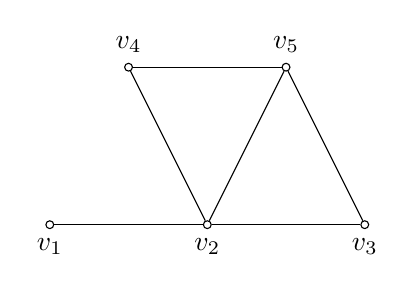
\begin{tikzpicture}
		% Nodes
		\node[draw, circle, inner sep=1pt, label=below:$v_1$] (v1) at (0,0) {};
		\node[draw, circle, inner sep=1pt, label=below:$v_2$] (v2) at (2,0) {};
		\node[draw, circle, inner sep=1pt, label=below:$v_3$] (v3) at (4,0) {};
		\node[draw, circle, inner sep=1pt, label=above:$v_4$] (v4) at (1,2) {};
		\node[draw, circle, inner sep=1pt, label=above:$v_5$] (v5) at (3,2) {};
		
		% Edges
		\draw (v1) -- (v2);
		\draw (v2) -- (v3);
		\draw (v2) -- (v4);
		\draw (v2) -- (v5);
		\draw (v3) -- (v5);
		\draw (v4) -- (v5);
	\end{tikzpicture}
\end{wrapfigure}
\textit{Маршрутом} в графе $G$ называется чередующаяся последовательность вершин и рёбер $v_0, x_1, v_1, \ldots, x_n, v_n$; эта последовательность начинается и кончается вершиной, и каждое ребро последовательности инцидентно двум вершинам, одна из которых непосредственно предшествует ему, а другая непосредственно следует за ним. Указанный маршрут соединяет вершины $v_0$ и $v_n$, и его можно обозначить $v_0 v_1 v_2 \ldots v_n$ (наличие рёбер подразумевается). Эта последовательность иногда называется $(v_0-v_n)$-маршрутом. Маршрут \textit{замкнут}, если $v_0 = v_n$, и \textit{открыт} в противном случае. Маршрут называется \textit{цепью} (trail), если все его рёбра различны, и \textit{простой цепью} (path), если все вершины (а следовательно, и рёбра) различны. Замкнутая цепь называется \textit{циклом}. Замкнутый маршрут называется \textit{простым циклом}, если все его $n$ вершин различны и $n \geq 3$.

В помеченном графе $G$ на рис. 2.9 $v_1 v_2 v_3 v_2 v_3$ — маршрут, который не является цепью, а $v_1 v_2 v_5 v_4 v_2 v_3$ — не простая цепь, $v_1 v_2 v_5 v_4$ — простая цепь и $v_2 v_4 v_5 v_2$ — простой цикл.

Длина маршрута $v_0 v_1 \ldots v_n$ равна $n$, т. е. количеству рёбер в нём\footnote{Обхват графа $G$ — обозначается $g(G)$ — это длина кратчайшего простого цикла графа $G$ (если он есть); окружение графа $G$ — обозначается $c(G)$ — длина самого длинного простого цикла графа $G$. Эти понятия не определены в случае, когда в $G$ нет циклов.}.